\documentclass[11pt]{article}

% Change "review" to "final" to generate the final (camera-ready) version.
\usepackage[review]{acl}

\usepackage{times}
\usepackage{latexsym}
\usepackage[T1]{fontenc}
\usepackage[utf8]{inputenc}
\usepackage{microtype}
\usepackage{graphicx}
\usepackage{booktabs}
\usepackage{multirow}
\usepackage{amsmath}
\usepackage{textcomp}

\title{IndiaFinBench: An Evaluation Benchmark for Large Language Model Performance on Indian Financial Regulatory Text}

\author{Anonymous ACL submission}

\begin{document}
\maketitle

\begin{abstract}
Financial NLP benchmarks test large language models almost exclusively against Western sources---SEC filings, US earnings reports, English-language financial news---leaving regulatory reasoning outside that context unmeasured. We introduce IndiaFinBench, a 406-item expert-annotated benchmark over SEBI and RBI regulatory text spanning four task types---regulatory interpretation, numerical reasoning, contradiction detection, and temporal reasoning---validated through a model-based secondary pass and a 180-item human inter-annotator study. Evaluating twelve contemporary LLMs zero-shot, strict string-matching accuracy ranges from 70.4\% to 89.7\%, and an item-level LLM-judge audit of every flagged error bounds semantically corrected accuracy at 79.8--96.6\%. The gap between scoring regimes is itself diagnostic: the reasoning-specialized DeepSeek R1 70B ranks 11th of twelve under strict scoring, yet the judge attributes 86\% of its errors to format non-compliance---evidence that accuracy conflates capability with its extraction under deployment-style constraints. Parameter efficiency holds under both regimes: Llama 4 Scout 17B matches LLaMA-3.3-70B with one-quarter the parameters, and GPT-OSS 120B gains nothing over its 20B sibling. The sharpest test is human, not architectural: on a 60-item medium-and-hard subset answered by a non-specialist evaluator (80.0\%), no model performs significantly better and only the weakest performs significantly worse---current LLMs match, not exceed, careful human judgment on the benchmark's hardest items.
\end{abstract}

\section{Introduction}

India's securities and banking regulators govern trillions of rupees in transactions through a body of circulars, master directions, and regulations that compliance teams, auditors, and retail investors must interpret correctly---a misread threshold or an overlooked amendment carries direct financial and legal consequence. Large language models are an increasingly plausible tool for this kind of regulatory reading, and evaluation benchmarks are the primary instrument by which the field measures whether that plausibility is warranted. In finance, this has produced a substantial body of work---FinQA \citep{chen2021finqa}, FinanceBench \citep{islam2023financebench}, PIXIU/FLARE \citep{xie2023pixiu}, and FinBen \citep{xie2024finben}, among others---testing models on numerical reasoning, document QA, and instruction-following across financial tasks. Virtually all of it, however, is built from US or European regulatory and corporate sources, leaving exactly this capability---reasoning about regulatory text outside the Western financial context---poorly characterized.

India's financial regulatory architecture---SEBI circulars, RBI monetary policy directives, and a dense network of amendment chains linking successive instruments---poses challenges that existing benchmarks do not capture. Indian regulatory text routinely embeds numerical thresholds directly in prose (capital adequacy ratios, upfront margin requirements, dividend payout limits), requires tracing chains of superseding circulars to resolve temporal questions, and uses jurisdiction-specific terminology (LODR, PMLA, SFB, AIF, FEMA) that models trained predominantly on Western corpora have little reason to have learned.

We introduce IndiaFinBench to make these challenges directly measurable.\footnote{Dataset, evaluation harness, and all model predictions: \url{https://anonymous.4open.science/r/IndiaFinBench-322D/}. De-anonymized upon acceptance.} The benchmark is built entirely from publicly available primary sources and validated through both a model-based secondary quality pass and an independent human inter-annotator agreement study spanning 180 items across three rounds (44.3\% benchmark coverage). One result previews the benchmark's diagnostic value: the reasoning-specialized DeepSeek R1 70B ranks 11th of twelve models under strict string-matching, yet an item-level semantic audit reclassifies 86\% of its errors as format non-compliance rather than incorrect reasoning (Section~\ref{sec:discussion})---a deployment-relevant failure mode that single-metric evaluation conflates with capability. Our contributions are:

\begin{enumerate}
\item A zero-shot evaluation of twelve contemporary LLMs under two scoring regimes---strict string-matching and an item-level LLM-judge audit of all 874 flagged errors---that brackets true accuracy and separates format non-compliance from reasoning failure, the paper's central methodological finding.
\item A paired human--model comparison on a 60-item subset showing that current LLMs match, rather than exceed, careful non-specialist human judgment on the benchmark's hardest items.
\item A new benchmark dataset of 406 expert-annotated QA pairs across four task types, drawn from 192 SEBI and RBI documents spanning 1992--2026.
\item Paired bootstrap significance analysis (10,000 resamples) under both scoring regimes, characterising which performance differences are statistically robust.
\item A validated annotation protocol achieving $\kappa$ = 0.645 on contradiction detection across 180 independent human judgments across three annotation rounds (44.3\% benchmark coverage), and a model-based secondary quality check (90.7\% agreement, 150-item subset).
\item An error taxonomy classifying model failures into four interpretable categories, providing actionable insight into where current models fail on Indian regulatory text.
\item Public release of the full dataset, evaluation harness, model predictions, and reproducibility code.
\end{enumerate}

\section{Related Work}

\subsection{Financial NLP Benchmarks}

The financial NLP community has built substantial evaluation infrastructure, but anchored almost entirely in Western financial text. FinQA \citep{chen2021finqa} and ConvFinQA \citep{zheng2022convfinqa} test numerical reasoning over SEC filings; FiNER-139 \citep{loukas2022finer} targets NER in the same filings; FLUE \citep{shah2022flue} packages several such tasks into a multi-task suite. PIXIU/FLARE \citep{xie2023pixiu} and FinBen \citep{xie2024finben}---the latter spanning 42 datasets across 24 tasks, including two aimed at financial regulation---push toward broader coverage, yet neither defines temporal or amendment-chain supersession reasoning as a task type, and both remain bounded by US and European sources. FinanceBench \citep{islam2023financebench}, closest in spirit to our work, evaluates financial document QA with human-verified gold answers, but over publicly listed US companies only. Geography, not task diversity, is the binding constraint this literature shares; to our knowledge, IndiaFinBench is the first publicly available benchmark targeting the Indian financial regulatory domain.

\subsection{Regulatory and Legal Text Understanding}

Legal-NLP benchmarks rarely address financial regulation: CUAD \citep{hendrycks2021cuad} targets contract clause extraction, LexGLUE \citep{chalkidis2022lexglue} European legal comprehension, and ILDC \citep{malik2021ildc} Indian court judgment prediction. Financial regulatory documents pose structural challenges this literature does not directly address---dense numerical thresholds embedded in prose, amendment chains where later instruments modify earlier ones, and domain-specific terminology with precise legal meaning. IndiaFinBench's four-task taxonomy makes each of these properties directly measurable under controlled QA conditions, complementing general-domain frameworks such as MMLU \citep{hendrycks2021mmlu} and HELM \citep{liang2022helm}.

\section{Dataset Construction}

Closing this gap requires building from Indian regulatory documents at a scale sufficient for reliable model comparison, while preserving the domain expertise that interpreting them demands---the constraint that shaped every design choice below.

\subsection{Source Document Collection}

We collected 192 regulatory documents spanning 1992--2026 from two official Indian government sources: the Securities and Exchange Board of India (92 documents: circulars, master circulars, regulations, orders; sebi.gov.in) and the Reserve Bank of India (100 documents: circulars, policy statements, directions; rbi.org.in). Documents were downloaded using a custom Python scraping pipeline and converted to clean text using pdfplumber, which handles the multi-column layouts and embedded tables common in Indian regulatory PDFs particularly well. Figure~\ref{fig:pipeline} (Appendix~\ref{app:examples}) illustrates the full dataset construction pipeline; Appendix~\ref{app:sourcedocs} lists the regulatory categories covered.

\subsection{Task Types}

IndiaFinBench defines four task types, each probing a distinct reasoning capability. Figure~\ref{fig:taskexamples} (Appendix~\ref{app:examples}) provides a representative example of each.

\textbf{Regulatory Interpretation (REG, 174 items).} Given a regulatory passage, identify the correct rule, compliance threshold, or scope of applicability---e.g., that a stock exchange must forward a registration application ``not later than thirty days of receipt.''

\textbf{Numerical Reasoning (NUM, 92 items).} Perform arithmetic over figures embedded in regulatory text---e.g., computing a Small Finance Bank's maximum eligible dividend from its Tier 1 Capital Ratio and adjusted profit after tax. Requires both correct extraction and arithmetic execution.

\textbf{Contradiction Detection (CON, 62 items).} Given two passages from different regulatory instruments, determine (Yes/No, with a one-sentence explanation) whether they contradict on the issue described---probing supersession tracking, a core challenge where circulars are frequently amended.

\textbf{Temporal Reasoning (TMP, 78 items).} Establish chronological ordering of regulatory events, identify which version of a rule was in force at a given time, or compute elapsed time between milestones. Indian regulatory documents frequently reference earlier instruments only by date, requiring a consistent regulatory timeline.

\subsection{Annotation Protocol}

All question-answer pairs were authored by the primary annotator, who has specialist experience with Indian financial regulatory documents. Expert single-annotator construction is standard for domain-specific benchmarks where annotation requires expertise unavailable to crowdsourced pools \citep{hendrycks2021cuad, malik2021ildc, islam2023financebench}; IndiaFinBench requires parallel familiarity with SEBI's securities regulation framework, RBI's prudential norms, and the amendment-chain structure linking hundreds of circulars over three decades. Section~\ref{sec:iaa} presents an independent human inter-annotator agreement study that empirically validates annotation quality. Each item consists of a context passage (80--500 words), a question, a reference answer, and metadata fields (task type, difficulty, source document).

Answer formats are standardized by task type: extractive spans for regulatory interpretation and temporal reasoning; calculated values with units for numerical reasoning (e.g., `Rs.~5,500 crore'); and `Yes' or `No' with a brief explanation for contradiction detection.

Difficulty levels were assigned by the number of reasoning steps required: easy items are single-step extraction (160 items, 39.4\%), medium items require multi-clause reasoning or calculation (182, 44.8\%), and hard items span multiple instruments or complex arithmetic (64, 15.8\%).

\textbf{Annotation scale rationale.} The 406-item scale is a deliberate quality-over-quantity decision: each item requires domain knowledge of SEBI circulars, RBI master directions, and their decade-spanning amendment chains, which is structurally incompatible with crowdsourcing. For context, FinanceBench released 150 expert-verified items \citep{islam2023financebench}. IndiaFinBench's 406 items span 192 source documents across 34 years and four task types, and the IAA study (Section~\ref{sec:iaa}) independently validates 44.3\% of all items.

Every item was individually reviewed to ensure: (1) the answer is unambiguously derivable from the provided context; (2) the question has exactly one correct answer; and (3) the context is sufficient without external knowledge.

\subsection{Model-Based Secondary Validation}

To confirm that items are unambiguously answerable from context, a secondary validation pass was conducted using LLaMA-3.3-70B-Versatile (via Groq API) as an independent quality-checker under a context-only, zero-shot prompt (temperature = 0). Although LLaMA-3.3-70B also appears in the main evaluation, the two uses are functionally distinct: the validation pass asks whether a question is unambiguously answerable from its context passage---a different task from the evaluation's open-ended QA. The validation endpoint was accessed in isolation from the evaluation pipeline, preventing cross-contamination of outputs.

Using a model-based validator as a tractability check follows established benchmark construction practice \citep{islam2023financebench, hendrycks2021cuad}.

\begin{table}[t]
\centering\small
\begin{tabular}{lrrrr}
\toprule
 & \multicolumn{2}{c}{\textbf{Model-based}} & \multicolumn{2}{c}{\textbf{Human IAA}} \\
\textbf{Task} & \textbf{Items} & \textbf{Agr.} & \textbf{Items} & \textbf{Agr.} \\
\midrule
REG & 53 & 85.7\% & 63 & 85.7\% \\
NUM & 32 & 84.4\% & 44 & 59.1\% \\
CON & 30 & 96.7\%\textsuperscript{$\kappa$=.918} & 35 & 88.6\%\textsuperscript{$\kappa$=.645} \\
TMP & 35 & 77.1\% & 38 & 73.7\% \\
\midrule
\textbf{All} & \textbf{150} & \textbf{90.7\%} & \textbf{180} & \textbf{77.2\%} \\
\bottomrule
\end{tabular}
\caption{Annotation validation: model-based secondary pass (150-item subset) and human inter-annotator agreement (180 items, three 60-item rounds, second annotator blind to reference answers). Cohen's $\kappa$ applies only to the binary CON task.}
\label{tab:validation}
\end{table}

The 90.7\% overall agreement rate (Table~\ref{tab:validation}, left) exceeds the 80\% threshold commonly used as a benchmark quality criterion. Items with genuine disagreement ($\sim$1.3\% of the initial set) were removed.

\subsection{Human Inter-Annotator Agreement}
\label{sec:iaa}

To provide rigorous empirical validation of single-annotator annotation quality, we conducted a human inter-annotator agreement (IAA) study in which a second independent human annotator completed three annotation rounds of 60 items each (180 items total; 44.3\% of the benchmark), drawn proportionally from all four task types and weighted toward medium and hard difficulty. The annotator worked from context passages and questions alone, without access to the primary annotator's reference answers at any stage.

Agreement was then computed between the primary annotator's reference answers and the second annotator's responses, using the same four-stage scoring procedure applied to model predictions (Section~\ref{sec:scoring}); results are in Table~\ref{tab:validation} (right).

The $\kappa$ = 0.645 for contradiction detection falls in the `substantial agreement' band by \citet{landiskoch1977} conventions, and is comparable to human agreement rates reported for similar binary contradiction detection tasks in legal NLP. The lower numerical reasoning agreement (59.1\%) reflects formatting conventions rather than substantive disagreement: reference answers often included intermediate calculation steps (e.g., `Rs.~19,000 crore maximum per Table~1 of the Directions'), whereas the second annotator provided only final values (`19,000 crore'). Post-hoc review of every discordant numerical item confirmed the computed values were equivalent in all cases; disagreements arose solely from intermediate-step presence, currency symbol style, and comma placement.

\section{Experimental Setup}

\subsection{Models}

We evaluate twelve models spanning a wide range of sizes, providers, and access modes on the full 406-item benchmark (Table~\ref{tab:models}, Appendix~\ref{app:models}): Gemini 2.5 Flash and Gemini 2.5 Pro (Google APIs); Qwen3-32B, LLaMA-3.3-70B, Llama 4 Scout 17B, Kimi K2, GPT-OSS 120B, GPT-OSS 20B, and DeepSeek R1 70B (Groq API); and LLaMA-3-8B, Mistral-7B, and Gemma 4 E4B run locally via Ollama v0.6.5 in 4-bit quantization (Q4\_K\_M) on an RTX 4060 (8~GB). All models were evaluated under identical zero-shot conditions with no fine-tuning or prompt adaptation; exact checkpoint identifiers are documented in the evaluation code.

\subsection{Prompting Strategy}

Our evaluation follows the extractive QA paradigm established by SQuAD \citep{rajpurkar2016squad}, in the same spirit as DROP's discrete-reasoning-over-text framing \citep{dua2019drop}, with context passages provided directly to the model under zero-shot, context-only constraints. This design isolates the model's ability to reason about regulatory text rather than recall memorized facts, making the benchmark robust to training data contamination. All models received a system prompt establishing the context-only constraint: ``You are an expert in Indian financial regulation and policy. Answer questions using ONLY the provided context passage. Do not use any external knowledge. Be concise and precise. Give only the answer---no preamble.'' Task-specific user prompts provided appropriate formatting instructions for each task type. For contradiction detection, both passages were labelled explicitly as `Passage A / Passage B'. For numerical reasoning, models were instructed to show calculation steps and include units---an instruction in tension with the system prompt's ``no preamble'' constraint, which contributes to the verbosity-related scoring penalty quantified in Appendix~\ref{app:judge}. All models were evaluated under identical prompting and decoding settings (temperature = 0.0; completion budget 200 tokens for API models, 300 for local models).

We evaluate exclusively under zero-shot conditions, as this most closely reflects practical deployment where users query models without domain-specific priming, and because it eliminates confounds from example selection strategy and ordering effects. Few-shot results for four top models are reported in Appendix~\ref{app:fewshot}.

\subsection{Scoring}
\label{sec:scoring}

Answers were scored using a multi-stage matching procedure applied in sequence: (1) exact match after case-normalization and punctuation stripping; (2) fuzzy token match using RapidFuzz \texttt{token\_set\_ratio} $\geq$ 0.72, applied when exact match fails, with the 0.72 threshold established by manual inspection of 20 borderline cases and validated against adjacent thresholds (0.65 and 0.80); (3) numerical extraction match, where the item is scored correct if the set of numbers extracted from both the reference and prediction are identical (handling currency symbols, comma separators, and units); and (4) Yes/No match for contradiction detection, comparing the leading word of the prediction to the reference.

To measure the false-negative rate of the automated pipeline, we applied a secondary LLM-as-judge validation using Gemini 2.5 Flash over items marked incorrect on NUM, REG, and TMP tasks across the twelve models. Of 935 flagged predictions, 874 were judged; the remaining 61 (58 empty responses and 3 API failures) are unambiguously incorrect and required no semantic review. CON items use exact Yes/No matching and were not judged. Judge reliability was confirmed on a 28-item stratified manual audit (89.3\% accuracy). Full results are in Appendix~\ref{app:judge}; primary Table~\ref{tab:mainresults} scores use the strict automated pipeline. DeepSeek R1 70B was accessed through an endpoint that returns final answers without exposed reasoning traces; its stored predictions contain no chain-of-thought markup, and its internal deliberation shares the fixed completion budget---a constraint we return to in Section~\ref{sec:discussion}.

\subsection{Human Reference Point}
\label{sec:humanbaseline}

To anchor model scores against human performance, a single non-specialist evaluator (a university-educated adult with no professional background in finance or law) independently answered 60 benchmark items sampled from the medium (40) and hard (20) difficulty strata across all four task types (REG 11, NUM 16, CON 17, TMP 16). The evaluator worked from the same context passages and questions given to the models, without access to reference answers or external resources, and responses were scored by the identical automated pipeline of Section~\ref{sec:scoring}. The evaluator scored 80.0\% (48/60; 95\% Wilson CI [68.2\%, 88.2\%]): REG 100\% (11/11), TMP 87.5\% (14/16), CON 82.4\% (14/17), NUM 56.2\% (9/16). Because the sample deliberately excludes easy items, this is a reference point for the benchmark's harder portion, not an estimate of whole-benchmark human accuracy; with one evaluator it reflects a single careful non-specialist rather than a population. Section~\ref{sec:humananalysis} compares each model to this reference on the identical 60 items using paired bootstrap tests.

\section{Results}

\subsection{Main Results}

\begin{table*}[t]
\centering\small
\begin{tabular}{lrrrrrl}
\toprule
\textbf{Model} & \textbf{REG} & \textbf{NUM} & \textbf{CON} & \textbf{TMP} & \textbf{Overall} & \textbf{95\% CI} \\
\midrule
Gemini 2.5 Flash & 93.1 & 84.8 & 88.7 & 88.5 & 89.7 & [86.3\%, 92.3\%] \\
Qwen3-32B & 85.1 & 77.2 & 90.3 & 92.3 & 85.5 & [81.7\%, 88.6\%] \\
LLaMA-3.3-70B & 86.2 & 75.0 & 95.2 & 79.5 & 83.7 & [79.8\%, 87.0\%] \\
Llama 4 Scout 17B & 86.2 & 66.3 & 98.4 & 84.6 & 83.3 & [79.3\%, 86.6\%] \\
Kimi K2 & 89.1 & 65.2 & 91.9 & 75.6 & 81.5 & [77.5\%, 85.0\%] \\
LLaMA-3-8B & 79.9 & 64.1 & 93.5 & 78.2 & 78.1 & [73.8\%, 81.8\%] \\
GPT-OSS 120B & 79.9 & 59.8 & 95.2 & 76.9 & 77.1 & [72.8\%, 80.9\%] \\
GPT-OSS 20B & 79.9 & 58.7 & 95.2 & 76.9 & 76.8 & [72.5\%, 80.7\%] \\
Gemini 2.5 Pro\textdagger{} & 89.7 & 48.9 & 93.5 & 64.1 & 76.1 & [71.7\%, 80.0\%] \\
Mistral-7B & 79.9 & 66.3 & 80.6 & 74.4 & 75.9 & [71.5\%, 79.8\%] \\
DeepSeek R1 70B & 72.4 & 69.6 & 96.8 & 70.5 & 75.1 & [70.7\%, 79.1\%] \\
Gemma 4 E4B & 83.9 & 50.0 & 72.6 & 62.8 & 70.4 & [65.8\%, 74.7\%] \\
\midrule
\textbf{Average} & \textbf{83.8} & \textbf{65.5} & \textbf{91.0} & \textbf{77.0} & \textbf{79.4} & --- \\
\bottomrule
\end{tabular}
\caption{IndiaFinBench results --- accuracy (\%) by task type under the strict string-matching pipeline. All twelve models evaluated on the full 406-item benchmark. 95\% Wilson score \citep{wilson1927} confidence intervals shown for overall accuracy. \textdagger{}Gemini 2.5 Pro evaluated via Vertex AI; lower NUM/TMP scores are a scoring artifact of its verbose output style (Section~\ref{sec:main-results-text}). Item-level judge-corrected accuracies, which bound semantic accuracy from above, are in Appendix~\ref{app:judge}.}
\label{tab:mainresults}
\end{table*}

\label{sec:main-results-text}
Gemini 2.5 Flash achieves the highest overall accuracy at 89.7\%, leading on both regulatory interpretation (93.1\%) and numerical reasoning (84.8\%). Its advantage over Qwen3-32B (85.5\%) is significant before multiple-comparison correction (bootstrap p = 0.041) but not after it (Section~\ref{sec:significance}). Qwen3-32B leads the temporal reasoning task (92.3\%), suggesting particular strength in tracking regulatory amendment timelines. Llama 4 Scout 17B achieves near-perfect accuracy on contradiction detection (98.4\%) despite its smaller size.

Gemini 2.5 Pro (76.1\%) underperforms the smaller Gemini 2.5 Flash (89.7\%) because its verbose outputs are penalized by exact-match scoring, especially on NUM (48.9\%) and TMP (64.1\%); judge-corrected scoring (Appendix~\ref{app:judge}) raises its overall accuracy to 95.1\%, eliminating essentially all of the apparent gap.

\textbf{Robustness to prompting strategy.} Under 3-shot prompting of the four top models, numerical reasoning improves by 2.1--16.3 percentage points and the top-cluster ordering is preserved, confirming that zero-shot scores are conservative for NUM and TMP without altering the comparative structure (Appendix~\ref{app:fewshot}).

\subsection{Human Reference Comparison}
\label{sec:humananalysis}

These numbers mean little without a reference point. Table~\ref{tab:mainresults} places all twelve models against a non-specialist human on the identical 60 medium-and-hard items (Section~\ref{sec:humanbaseline}), using the same paired bootstrap procedure applied to the model-vs-model comparisons below. The result is symmetric and sobering: no model significantly outperforms the human (best: Gemini 2.5 Flash, 85.0\% vs.\ 80.0\%, p = 0.48), and only the weakest model is significantly worse (Gemma 4 E4B, 63.3\%, p = 0.011). On the harder portion of the benchmark, current LLMs cluster around---not above---careful non-specialist judgment; with one evaluator and 60 items this is a reference point rather than a population estimate, and a domain specialist would likely score higher still.

The task-level contrast is sharper than the aggregate. The human scored 100\% on regulatory interpretation---reading a passage and extracting the governing rule is something a careful adult does reliably---but 56.2\% on numerical reasoning. Models show the opposite gradient: the best exceed the human by nearly 30 points on NUM (84.8\% vs.\ 56.2\%) while merely matching human-level REG extraction. Multi-step numerical inference over embedded regulatory thresholds is therefore the benchmark's one capability where models decisively exceed a careful human---and, as the task-level analysis confirms (Section~\ref{sec:tasklevel}), its most discriminating task among models themselves.

\subsection{Statistical Significance and Performance Tiers}
\label{sec:significance}

Paired bootstrap significance testing (10,000 resamples) across all 66 model pairs finds 42 pairs significantly different at p $<$ 0.05, of which 19 survive Bonferroni correction ($\alpha$ = 0.05/66 $\approx$ 0.00076). Three descriptive performance clusters organize the results; as detailed below, their boundaries are robust at the top and bottom of the ranking but statistical, not categorical, in the middle.

\textbf{Tier 1} --- strong performers (81.5--89.7\%): Gemini 2.5 Flash, Qwen3-32B, LLaMA-3.3-70B, Llama 4 Scout 17B, and Kimi K2. Gemini 2.5 Flash sits measurably above the rest of this tier (p = 0.041 vs.\ Qwen3-32B, p $\leq$ 0.005 vs.\ the other three), while Qwen3-32B, LLaMA-3.3-70B, Llama 4 Scout 17B, and Kimi K2 are mutually indistinguishable (p = 0.06--0.80), forming a genuine performance plateau. Llama 4 Scout 17B is statistically indistinguishable from LLaMA-3.3-70B despite a four-fold parameter difference (p = 0.80).

\textbf{Tier 2} --- middle performers (75--79\%): LLaMA-3-8B, GPT-OSS 120B, GPT-OSS 20B, Gemini 2.5 Pro, Mistral-7B, and DeepSeek R1 70B. GPT-OSS 120B (77.1\%) and GPT-OSS 20B (76.8\%) are statistically indistinguishable (p = 0.861) despite a six-fold size difference, and LLaMA-3-8B and Mistral-7B are tied (p = 0.355).

\textbf{Tier 3}: Gemma 4 E4B stands alone at 70.4\%, driven by near-chance numerical reasoning (50.0\%) and the lowest contradiction detection score (72.6\%).

The tier boundaries are not uniformly significant, and we flag the exceptions explicitly. Every Tier 1 model separates from Gemma 4 E4B at the Bonferroni threshold (all p $<$ 0.0001), and nearly all Tier 1 vs.\ Tier 2 pairs are significant at p $<$ 0.05 (29 of 30, with 13 surviving Bonferroni). But Gemma 4 E4B is \emph{not} significantly below Mistral-7B (p = 0.072) or DeepSeek R1 70B (p = 0.110), and Kimi K2 is not significantly above LLaMA-3-8B (p = 0.147). The robust statistical statement is therefore top-versus-bottom separation---the strongest five models versus the weakest---with a graded middle, rather than three categorically distinct tiers. Full pairwise p-values under both scoring regimes are released with the evaluation code.

\subsection{Task-Level Analysis}
\label{sec:tasklevel}

Regulatory Interpretation (REG) shows a 20.7 percentage-point spread (Gemini: 93.1\% vs DeepSeek R1 70B: 72.4\%). All frontier API models exceed 85\% on this task. DeepSeek R1 70B's low REG score is where the strict pipeline penalizes its reasoning-style output most heavily: the semantic judge reclassifies the large majority of its REG errors as format mismatches (corrected REG: 95.4\%, Appendix~\ref{app:judge}), indicating misalignment between chain-of-thought output style and extractive, precision-dependent scoring rather than missing domain knowledge.

Numerical Reasoning (NUM) is the most discriminative task, with a 35.9 percentage-point spread (Gemini 2.5 Flash: 84.8\% vs Gemini 2.5 Pro: 48.9\%)---the same task on which Section~\ref{sec:humananalysis} found models decisively outpace a careful human. As discussed, Gemini 2.5 Pro's low NUM score reflects a scoring artifact of its verbose output style. Among non-reasoning models, Gemma 4 E4B (50.0\%) is at near-chance level. The GPT-OSS models also underperform on NUM (59.8\% and 58.7\%), suggesting this family struggles with multi-step arithmetic over Indian regulatory text.

Contradiction detection shows the strongest average accuracy (91.0\%), but the task is class-imbalanced---85.5\% of items carry the gold label `No'---so the majority-class baseline is 85.5\%, not 50\%. Ten of twelve models exceed that baseline; Llama 4 Scout 17B leads at 98.4\%, 12.9 points above it. Balanced accuracy (mean of sensitivity and specificity) per model is reported in Appendix~\ref{app:con}.

Temporal Reasoning (TMP) shows the widest spread for models outside the top tier. Qwen3-32B leads at 92.3\%, while Gemma 4 E4B (62.8\%) and DeepSeek R1 70B (70.5\%) trail under strict scoring. The two low scores have different causes: Gemma 4 E4B's deficit persists under judge-corrected scoring (80.8\%), marking a genuine capability gap, whereas DeepSeek R1 70B's corrected TMP accuracy reaches 98.7\%---its strict-scoring deficit on this task, like on REG, is overwhelmingly format non-compliance.

\subsection{Difficulty Analysis}

Per-model accuracy by difficulty level (full table and figure in Appendix~\ref{app:difficulty}) reveals contrasting behaviors: Gemini 2.5 Flash declines most sharply from easy to hard items (92.5\% $\rightarrow$ 84.4\%), while LLaMA-3.3-70B improves on hard items (79.4\% $\rightarrow$ 90.6\%), consistent with hard items' explicit amendment-chain cues rewarding capacity differently than medium items' subtler multi-clause reasoning. Gemma 4 E4B collapses from 82.5\% (easy) to 56.2\% (hard)---the signature of a small model that has absorbed common regulatory patterns but lacks multi-step reasoning capacity. Qwen3-32B and Kimi K2 are the most consistent across difficulty levels.

Difficulty explains \emph{how much} accuracy drops; it does not say \emph{why}. We turn to an error taxonomy to characterize the failures directly.

\section{Error Analysis}
\label{sec:errortax-sub}

\subsection{Error Taxonomy}

We classify model failures into four interpretable error types via a deterministic mapping from item task type and difficulty (released with the evaluation code; contradiction-detection errors map to TRF because the task probes supersession tracking, and hard REG items map to CGF):

\textbf{Domain Knowledge Failure (DKF)}: unfamiliarity with Indian regulatory concepts, terminology, or thresholds. \textbf{Numerical Reasoning Failure (NRF)}: arithmetic errors---wrong calculation, unit conversion, or formula application despite the formula appearing in context. \textbf{Temporal Reasoning Failure (TRF)}: mis-ordering regulatory events, misidentifying the circular in force at a given time, or failing to track supersession. \textbf{Context Grounding Failure (CGF)}: using external knowledge instead of the passage, or failing to extract a span clearly present in context.

Table~\ref{tab:errortax} shows error distributions for five key models under both scoring regimes: strict-pipeline errors, and residual errors that survive the item-level judge audit (Appendix~\ref{app:judge}). The distinction matters because strict errors mix true failures with format mismatches, whereas residual errors are the judge-confirmed failures.

\begin{table*}[t]
\centering\small
\begin{tabular}{llrrrrr}
\toprule
\textbf{Model} & \textbf{Errors} & \textbf{DKF} & \textbf{NRF} & \textbf{TRF} & \textbf{CGF} & \textbf{Total} \\
\midrule
\multirow{2}{*}{Gemini 2.5 Flash} & strict & 12 (29\%) & 14 (33\%) & 14 (33\%) & 2 (5\%) & 42 \\
 & residual & 6 (33\%) & 2 (11\%) & 10 (56\%) & 0 (0\%) & 18 \\
\multirow{2}{*}{Qwen3-32B} & strict & 25 (42\%) & 21 (36\%) & 11 (19\%) & 2 (3\%) & 59 \\
 & residual & 4 (24\%) & 5 (29\%) & 7 (41\%) & 1 (6\%) & 17 \\
\multirow{2}{*}{LLaMA-3.3-70B} & strict & 25 (38\%) & 23 (35\%) & 18 (27\%) & 0 (0\%) & 66 \\
 & residual & 4 (22\%) & 7 (39\%) & 7 (39\%) & 0 (0\%) & 18 \\
\multirow{2}{*}{DeepSeek R1 70B} & strict & 51 (50\%) & 28 (28\%) & 19 (19\%) & 3 (3\%) & 101 \\
 & residual & 7 (50\%) & 3 (21\%) & 2 (14\%) & 2 (14\%) & 14 \\
\multirow{2}{*}{Gemma 4 E4B} & strict & 29 (24\%) & 46 (38\%) & 43 (36\%) & 2 (2\%) & 120 \\
 & residual & 18 (22\%) & 33 (40\%) & 29 (35\%) & 2 (2\%) & 82 \\
\bottomrule
\end{tabular}
\caption{Error distribution by type for five key models under strict scoring and after judge correction (residual). DKF: Domain Knowledge Failure; NRF: Numerical Reasoning Failure; TRF: Temporal Reasoning Failure; CGF: Context Grounding Failure. Models selected as top performer (Gemini 2.5 Flash), bottom performer (Gemma 4 E4B), and three distinctive profiles. Counts derive from the released rule-based mapping and per-item judge verdicts; CON errors (mapped to TRF) are not judge-reviewed, so they persist into the residual column.}
\label{tab:errortax}
\end{table*}

Three patterns emerge. First, for top-tier models the judge audit removes most numerical and domain-knowledge errors as format artifacts, leaving temporal-supersession failures as the largest residual category (Gemini 2.5 Flash: 56\%, Qwen3-32B: 41\%, LLaMA-3.3-70B: 39\%)---though residual totals are small (17--18 items), so these shares are indicative rather than precise. Second, DeepSeek R1 70B's 101 strict errors collapse to 14 residual errors (86\% reclassified as format non-compliance), the largest correction of any model; its strict-error profile says more about its output format than its reasoning. Third, Gemma 4 E4B's errors barely move (120 $\rightarrow$ 82), confirming a genuine capability gap concentrated in numerical reasoning. Context Grounding Failure is rare in every regime.

Representative failure examples for each error type are given in Appendix~\ref{app:examples}.

\section{Discussion and Conclusion}
\label{sec:discussion}

IndiaFinBench's most actionable finding is not which model wins, but what winning means once scoring is held to account. DeepSeek R1 70B illustrates this most sharply: a 70B reasoning-specialized model that ranks last of twelve under strict extractive scoring, yet whose judge-corrected accuracy (96.6\%) is statistically indistinguishable from the top cluster once its 86\% format-driven errors are set aside (Section~\ref{sec:errortax-sub}). Our system prompt instructs models to answer without preamble, and completion budgets were fixed---conditions that work against a model whose signature behavior is extended visible reasoning, so we state the result's scope honestly rather than as an unqualified capability ranking. The correct conclusion is not that reasoning specialization fails at Indian regulatory reasoning; it is that reasoning-style output fails \emph{deployment-style extractive pipelines}, exactly the constrained, format-sensitive conditions a compliance workflow imposes. For practitioners selecting models for regulatory automation, that distinction between capability and extractable capability matters more than either scoring regime's raw leaderboard.

The same accounting clarifies why performance does not track parameter count. Llama 4 Scout 17B matches LLaMA-3.3-70B (83.3\% vs.\ 83.7\%, p = 0.80) with one-quarter the parameters, and GPT-OSS 120B gains nothing over its 20B sibling (77.1\% vs.\ 76.8\%, p = 0.861) despite a six-fold size difference. Both null results persist under judge-corrected scoring (p = 0.697 and p = 0.176), ruling out the possibility that a scoring artifact---rather than architecture---was masking a size effect: once a model clears a basic competence threshold on this benchmark, output-format alignment with extractive regulatory QA determines rank, not scale.

Held against a non-specialist human on the benchmark's hardest items (Section~\ref{sec:humananalysis}), current models do not clear a categorically higher bar either: no model significantly outperforms the human, and only the weakest is significantly worse. The one capability where models decisively pull ahead---multi-step numerical reasoning, where the best model exceeds the human by nearly 30 points---is also the benchmark's most discriminating task among models themselves, suggesting numerical inference over embedded regulatory thresholds is where genuine model capability, rather than scale or reasoning-style output, currently separates itself from a careful human reader.

IndiaFinBench's contribution is therefore less a leaderboard than a diagnostic instrument: a benchmark whose two scoring regimes and human reference point together show that Indian financial regulatory reasoning is not solved by size, and that evaluating it honestly requires distinguishing what a model knows from what a deployment pipeline can extract. Extending that instrument to India's other regulators---IRDAI, PFRDA, and commodity-segment regulation---and making semantically-aware scoring a first-class part of benchmark design, rather than a post-hoc audit, are the two directions we consider most likely to matter next.

\section*{Limitations}

Several limitations should be noted. The automated four-stage scoring pipeline penalizes semantically correct predictions that differ in number format (`50\%' vs `fifty per cent') or verbosity; the LLM-as-judge audit (Appendix~\ref{app:judge}) reclassifies 78.4\% of flagged items as correct. Neither regime is ground truth: strict scores under-count (format false negatives), while judge-corrected scores likely over-count, since the judge's confirmed error mode is over-crediting correct intermediate reasoning that reaches a wrong final answer (3 of 28 audited verdicts). True accuracy lies between the two bounds we report. The benchmark also does not cover Hindi--English code-switched regulatory text that appears in some official documents.

The human reference study involves a single non-specialist evaluator on 60 medium-and-hard items; it anchors the harder half of the benchmark but supports no population-level claims about human performance, and a domain specialist would likely score higher. The IAA study covers 180 of 406 items (44.3\%) across three rounds with CON agreement stable at $\kappa$ = 0.645; agreement on open-ended tasks reflects the same verbosity artifact documented in Appendix~\ref{app:judge}. Few-shot evaluation was conducted on only four top-performing models (Appendix~\ref{app:fewshot}). Judge-corrected significance tests reuse the judge's verdicts, so correlated judge errors could bias those comparisons; the strict-pipeline results carry no such dependence.

A structural limitation shared across all evaluations is context-injection: models receive the relevant passage directly rather than retrieving it from the full document corpus, testing reading comprehension over a provided excerpt rather than the retrieval or full-document understanding real-world compliance workflows also require. The benchmark is a static snapshot of SEBI and RBI regulation as of early 2026 and will need periodic refresh as the regulatory landscape evolves.

Primary annotation was conducted by a single domain-expert annotator, with the independent human inter-annotator study above providing external validation. All questions and gold-standard answers are in English; the official Hindi-language versions of the same circulars are not included, limiting applicability to multilingual regulatory analysis. Coverage is also limited to two regulators---extending to the Insurance Regulatory and Development Authority of India (IRDAI), the Pension Fund Regulatory and Development Authority (PFRDA), and commodity-segment regulation would substantially broaden the benchmark's coverage of the Indian financial regulatory ecosystem.

Finally, IndiaFinBench evaluates short extractive responses rather than longer-form generation; it does not test whether models can draft regulatory summaries, identify compliance gaps, or produce legally coherent reasoning chains---capabilities that are arguably more consequential for legal-technology applications and a natural next step for the benchmark.

\section*{Ethics Statement}

IndiaFinBench is constructed entirely from publicly available primary source documents released by the Securities and Exchange Board of India (sebi.gov.in) and the Reserve Bank of India (rbi.org.in). These documents are published by the Government of India for public use and carry no copyright restrictions on research use. No personally identifiable information is present in any source document or derived annotation. The benchmark is designed to evaluate model performance on regulatory reasoning tasks and does not contain any toxic, harmful, or privacy-violating content. The dataset is released under CC BY 4.0 to enable open research use with attribution.

% Acknowledgements are omitted from the anonymized review version per ACL
% double-blind policy. Restore this section for the camera-ready.
% \section*{Acknowledgements}
% Evaluation infrastructure used the Groq API (LLaMA-3.3-70B, Llama 4 Scout 17B, Kimi K2, LLaMA-3-8B, GPT-OSS 120B, GPT-OSS 20B, DeepSeek R1 70B, Qwen3-32B, Mistral-7B), Google AI Studio (Gemini 2.5 Flash), and Google Cloud Vertex AI (Gemini 2.5 Pro). Local model inference used Ollama (Gemma 4 E4B).

\bibliography{indiafinbench}

\appendix

\section{Source Document Categories}
\label{app:sourcedocs}

\textbf{SEBI Documents:} SEBI (Issue of Capital and Disclosure Requirements) Regulations 2018, SEBI (Listing Obligations and Disclosure Requirements) Regulations 2015, SEBI (Substantial Acquisition of Shares and Takeovers) Regulations 2011, SEBI (Prohibition of Insider Trading) Regulations 2015, SEBI (Alternative Investment Funds) Regulations 2012, SEBI (Portfolio Managers) Regulations 2020, SEBI (Research Analysts) Regulations 2014, SEBI (Buy-Back of Securities) Regulations 2018, SEBI (Delisting of Equity Shares) Regulations 2021, SEBI (Mutual Funds) Regulations 1996, SEBI (Depositories and Participants) Regulations 2018, SEBI (Merchant Bankers) Regulations 1992, recent SEBI circulars (2024--2026).

\textbf{RBI Documents:} RBI Monetary Policy Statements (2024--2026), RBI Master Directions on Unique Identifiers in Financial Markets, RBI (Small Finance Banks---Prudential Norms on Declaration of Dividend) Directions 2026, Government Securities auction notifications (2025--2026), State Government securities auction press releases, RBI Weekly Statistical Supplement extracts, RBI circulars on KYC/AML compliance.

\section{System Prompt Template}
\label{app:prompt}

\begin{quote}
\noindent You are an expert in Indian financial regulation and policy. Answer questions using ONLY the provided context passage. Do not use any external knowledge. Be concise and precise. Give only the answer --- no preamble.
\end{quote}

\section{CON Task: Majority-Class Baseline and Balanced Accuracy}
\label{app:con}

The contradiction detection task (CON) has a class-imbalanced label distribution: 53 of 62 items (85.5\%) carry the gold label `No' (no contradiction exists), yielding a majority-class baseline accuracy of 85.5\%. Table~\ref{tab:c1} reports raw CON accuracy, margin over that baseline, and balanced accuracy (mean of sensitivity and specificity) computed from each model's per-item predictions. All models except Gemma 4 E4B and Mistral-7B exceed the majority-class baseline. Balanced accuracy preserves the raw-accuracy ordering; notably, most models detect the nine true contradictions perfectly (sensitivity 100\%) and differ mainly in false-positive rate on the 53 `No' items.

\begin{table}[t]
\centering\small
\begin{tabular}{lrrr}
\toprule
\textbf{Model} & \textbf{CON \%} & \textbf{vs. Base} & \textbf{Bal. Acc.} \\
\midrule
Gemini 2.5 Flash & 88.7 & +3.2 & 88.8 \\
Qwen3-32B & 90.3 & +4.8 & 94.3 \\
LLaMA-3.3-70B & 95.2 & +9.7 & 97.2 \\
Llama 4 Scout 17B & 98.4 & +12.9 & 99.1 \\
Kimi K2 & 91.9 & +6.4 & 95.3 \\
LLaMA-3-8B & 93.5 & +8.0 & 91.6 \\
GPT-OSS 120B & 95.2 & +9.7 & 97.2 \\
GPT-OSS 20B & 95.2 & +9.7 & 97.2 \\
Gemini 2.5 Pro & 93.5 & +8.0 & 91.6 \\
Mistral-7B & 80.6 & $-$4.9 & 88.7 \\
DeepSeek R1 70B & 96.8 & +11.3 & 98.1 \\
Gemma 4 E4B & 72.6 & $-$12.9 & 74.7 \\
\midrule
Majority baseline & 85.5 & --- & 50.0 \\
\bottomrule
\end{tabular}
\caption{CON task raw accuracy, margin over the majority-class baseline (85.5\%), and balanced accuracy (mean of sensitivity and specificity over 9 `Yes' / 53 `No' gold labels).}
\label{tab:c1}
\end{table}

\section{Scoring Pipeline Validation}
\label{app:judge}

The automated scoring pipeline (Section~\ref{sec:scoring}) uses four stages: exact match, fuzzy token matching (RapidFuzz \texttt{token\_set\_ratio} $\geq$ 0.72), numerical extraction match, and Yes/No match for contradiction detection. While rigorous, the pipeline penalizes answers that are semantically correct but formatted differently from the reference answer---a systematic limitation of string-based matching for open-ended regulatory QA.

\subsection{Judge Validation Study}

To quantify this false-negative rate, we applied Gemini 2.5 Flash as a semantic judge over items marked incorrect across the twelve models on NUM, REG, and TMP task types. The strict pipeline flagged 935 such predictions; 874 were judged, and the remaining 61 (58 empty responses, 3 API failures) were retained as incorrect without review, since no semantic judgment can rescue an empty prediction. CON items use exact Yes/No matching and require no secondary validation. The judge received the question, reference answer, and model prediction, and returned CORRECT or INCORRECT with a one-sentence rationale.

Judge reliability was estimated on a stratified 28-item manual audit (20 NUM, 5 REG, 3 TMP). Manual review confirmed 25 of 28 verdicts (89.3\%) as correct. The three judge errors all involved multi-step numerical problems where the model showed correct intermediate reasoning but reached a wrong final answer (NUM\_074: predicted Rs.~19,000 crore vs.\ reference Rs.~33,000 crore; NUM\_103: concluded wrong direction for a threshold comparison; NUM\_136: applied wrong regulatory fee slab). These errors reflect the judge's tendency to over-credit partial reasoning chains on NUM items.

\subsection{Results}

Across 874 judged predictions, the judge reclassified 685 from incorrect to correct---an overall flip rate of 78.4\% (REG: 261/327 = 79.8\%; NUM: 272/348 = 78.2\%; TMP: 152/199 = 76.4\%). Table~\ref{tab:d1} presents corrected accuracies computed directly from the item-level verdicts: a prediction counts as correct if the strict pipeline accepted it or the judge reclassified it, over the full 406-item denominator. No aggregate correction formula is involved, and every value is exactly reproducible from the released per-item audit log.

\subsection{Root Causes}

Three systematic causes account for the majority of false negatives: (1) \textit{Numeric format differences} --- models frequently use digits (`50\%', `365 days') while references use written numbers (`fifty per cent', `three hundred and sixty-five days'). (2) \textit{Verbose answers} --- models prefix the correct answer with calculation steps or regulatory citations. (3) \textit{Abbreviated answers} --- models give a shorter but correct version of the reference (e.g., ref = `Six months after completion of the open offer'; pred = `Six months').

\subsection{Interpretation}

The two scoring regimes bracket true accuracy: strict scores under-count because of format false negatives, while judge-corrected scores likely over-count, given the judge's audited tendency to over-credit correct intermediate reasoning that reaches a wrong final answer. The two regimes tell substantively different stories, and we report both rather than claiming invariance. Under correction, eleven of twelve models converge to 90.6--96.6\% and are largely statistically indistinguishable; only Gemma 4 E4B (79.8\%) remains separated from every other model (all pairwise p $<$ 0.05, paired bootstrap on corrected labels). Of the 42 pairwise comparisons significant under strict scoring, 18 remain significant under corrected scoring. The strict-scoring tier structure of Section~\ref{sec:significance} is therefore a property of format-sensitive evaluation---which is exactly the deployment condition it models---while corrected scoring shows that the underlying semantic capability of current mid-size and frontier models on this benchmark is far more uniform, with the notable exception of Gemma 4 E4B's persistent numerical deficit. Item-level verdicts and judge-corrected CSVs are released at \texttt{evaluation/results\_judged/} in the repository.

\begin{table*}[t]
\centering\footnotesize
\begin{tabular}{lcccccc}
\toprule
\textbf{Model} & \textbf{REG} & \textbf{NUM} & \textbf{CON} & \textbf{TMP} & \textbf{Overall} \\
 & \textit{rep./corr.} & \textit{rep./corr.} & \textit{rep./corr.} & \textit{rep./corr.} & \textit{rep./corr.} \\
\midrule
Gemini 2.5 Flash & 93.1/97.1 & 84.8/97.8 & 88.7/88.7 & 88.5/94.9 & 89.7/95.6 \\
Qwen3-32B & 85.1/97.1 & 77.2/94.6 & 90.3/90.3 & 92.3/98.7 & 85.5/95.8 \\
LLaMA-3.3-70B & 86.2/97.7 & 75.0/92.4 & 95.2/95.2 & 79.5/94.9 & 83.7/95.6 \\
Llama 4 Scout 17B & 86.2/96.6 & 66.3/94.6 & 98.4/98.4 & 84.6/94.9 & 83.3/96.1 \\
Kimi K2 & 89.1/98.9 & 65.2/93.5 & 91.9/91.9 & 75.6/96.2 & 81.5/96.1 \\
LLaMA-3-8B & 79.9/94.3 & 64.1/84.8 & 93.5/93.5 & 78.2/91.0 & 78.1/91.4 \\
GPT-OSS 120B & 79.9/96.0 & 59.8/93.5 & 95.2/95.2 & 76.9/97.4 & 77.1/95.6 \\
GPT-OSS 20B & 79.9/96.6 & 58.7/92.4 & 95.2/95.2 & 76.9/88.5 & 76.8/93.8 \\
Gemini 2.5 Pro & 89.7/97.1 & 48.9/94.6 & 93.5/93.5 & 64.1/92.3 & 76.1/95.1 \\
Mistral-7B & 79.9/98.3 & 66.3/82.6 & 80.6/80.6 & 74.4/91.0 & 75.9/90.6 \\
DeepSeek R1 70B & 72.4/95.4 & 69.6/96.7 & 96.8/96.8 & 70.5/98.7 & 75.1/96.6 \\
Gemma 4 E4B & 83.9/90.2 & 50.0/64.1 & 72.6/72.6 & 62.8/80.8 & 70.4/79.8 \\
\bottomrule
\end{tabular}
\caption{Reported (rep.) and judge-corrected (corr.) accuracies (\%) by task, computed item-by-item from the released audit log: corrected-correct = pipeline-correct $\cup$ judge-flipped, over the full 406-item denominator. CON was not judge-reviewed, so its values are identical in both regimes. Corrected values are an optimistic bound (see Interpretation); the strict and corrected columns bracket true accuracy.}
\label{tab:d1}
\end{table*}

\section{Evaluated Models}
\label{app:models}

\begin{table}[t]
\centering\footnotesize
\begin{tabular}{lp{2.4cm}p{1.5cm}}
\toprule
\textbf{Model} & \textbf{Provider / Access} & \textbf{Params} \\
\midrule
Gemini 2.5 Flash & Google (AI Studio API) & --- \\
Gemini 2.5 Pro & Google (Vertex AI) & --- \\
Qwen3-32B & Alibaba (Groq API) & 32B \\
LLaMA-3.3-70B & Meta (Groq API) & 70B \\
Llama 4 Scout 17B & Meta (Groq API) & 17B \\
Kimi K2 & Moonshot AI (Groq API) & 1T total, 32B active (MoE) \\
LLaMA-3-8B & Meta (Ollama, local) & 8B \\
GPT-OSS 120B\textdaggerdbl{} & OpenAI (open-weight, Groq API) & 120B \\
GPT-OSS 20B\textdaggerdbl{} & OpenAI (open-weight, Groq API) & 20B \\
Mistral-7B & Mistral AI (Ollama, local) & 7B \\
DeepSeek R1 70B & DeepSeek (Groq API) & 70B \\
Gemma 4 E4B & Google (Ollama, local) & 4B \\
\bottomrule
\end{tabular}
\caption{Models evaluated in this study. \textdaggerdbl{}OpenAI open-weight models accessed via the Groq inference API. Local models ran on an Intel i7-13650HX CPU with an NVIDIA RTX 4060 GPU (8~GB VRAM); exact identifiers were \texttt{llama3:8b}, \texttt{mistral:7b}, and \texttt{gemma3:4b}, with temperature 0.0 via the Ollama REST API.}
\label{tab:models}
\end{table}

\section{Task Examples, Pipeline, and Failure Cases}
\label{app:examples}

Figure~\ref{fig:pipeline} illustrates the dataset construction pipeline. Figure~\ref{fig:taskexamples} shows a representative item for each task type; Figure~\ref{fig:heatmap} visualizes per-task accuracy across all twelve models.

\begin{figure*}[t]
\centering

\includegraphics[width=0.85\textwidth]{figures/fig_pipeline.png}
\caption{IndiaFinBench dataset construction pipeline. Starting from 192 SEBI and RBI PDFs (1992--2026), documents are parsed using pdfplumber and expert-annotated into 406 QA items across four task types (REG: 174, NUM: 92, CON: 62, TMP: 78). Quality is validated through a model-based secondary pass ($\kappa$ = 0.918 on CON; 90.7\% overall) and a 180-item human inter-annotator agreement study ($\kappa$ = 0.645 on CON; 77.2\% overall), yielding a benchmark evaluated on 12 models under zero-shot conditions.}
\label{fig:pipeline}
\end{figure*}

\begin{figure*}[t]
\centering
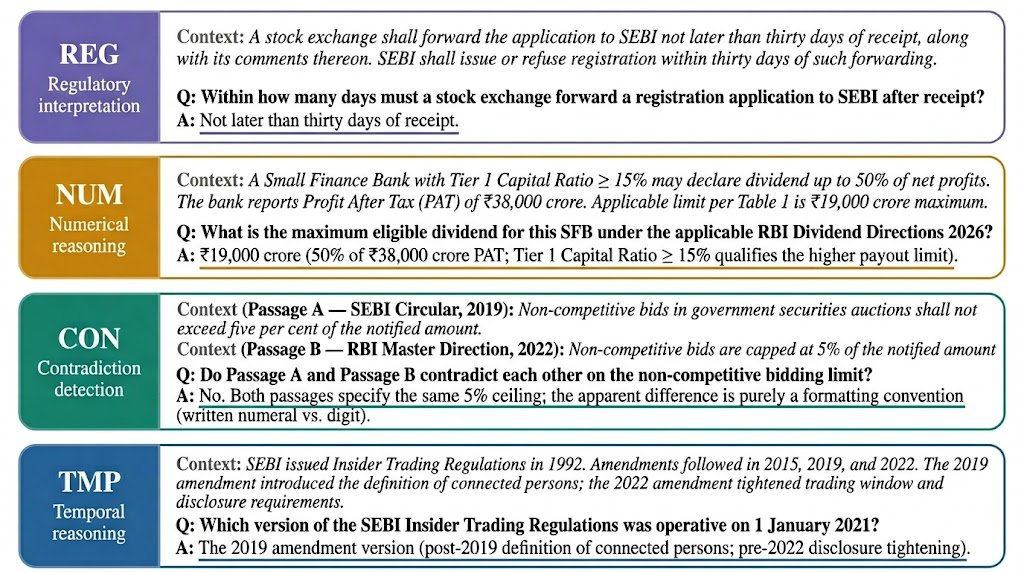
\includegraphics[width=0.85\textwidth]{figures/fig_taskexamples.png}
\caption{Representative examples of all four IndiaFinBench task types. REG (regulatory interpretation): the model extracts the correct compliance deadline from a SEBI passage. NUM (numerical reasoning): the model computes the maximum dividend payout for a Small Finance Bank using RBI Dividend Directions 2026, requiring multi-step arithmetic. CON (contradiction detection): the model determines whether two regulatory passages conflict, identifying that a surface-level phrasing difference (written numeral vs. digit) does not constitute a substantive contradiction. TMP (temporal reasoning): the model identifies the operative version of SEBI Insider Trading Regulations at a specific historical date. Reference answers are underlined.}
\label{fig:taskexamples}
\end{figure*}

\begin{figure}[t]
\centering
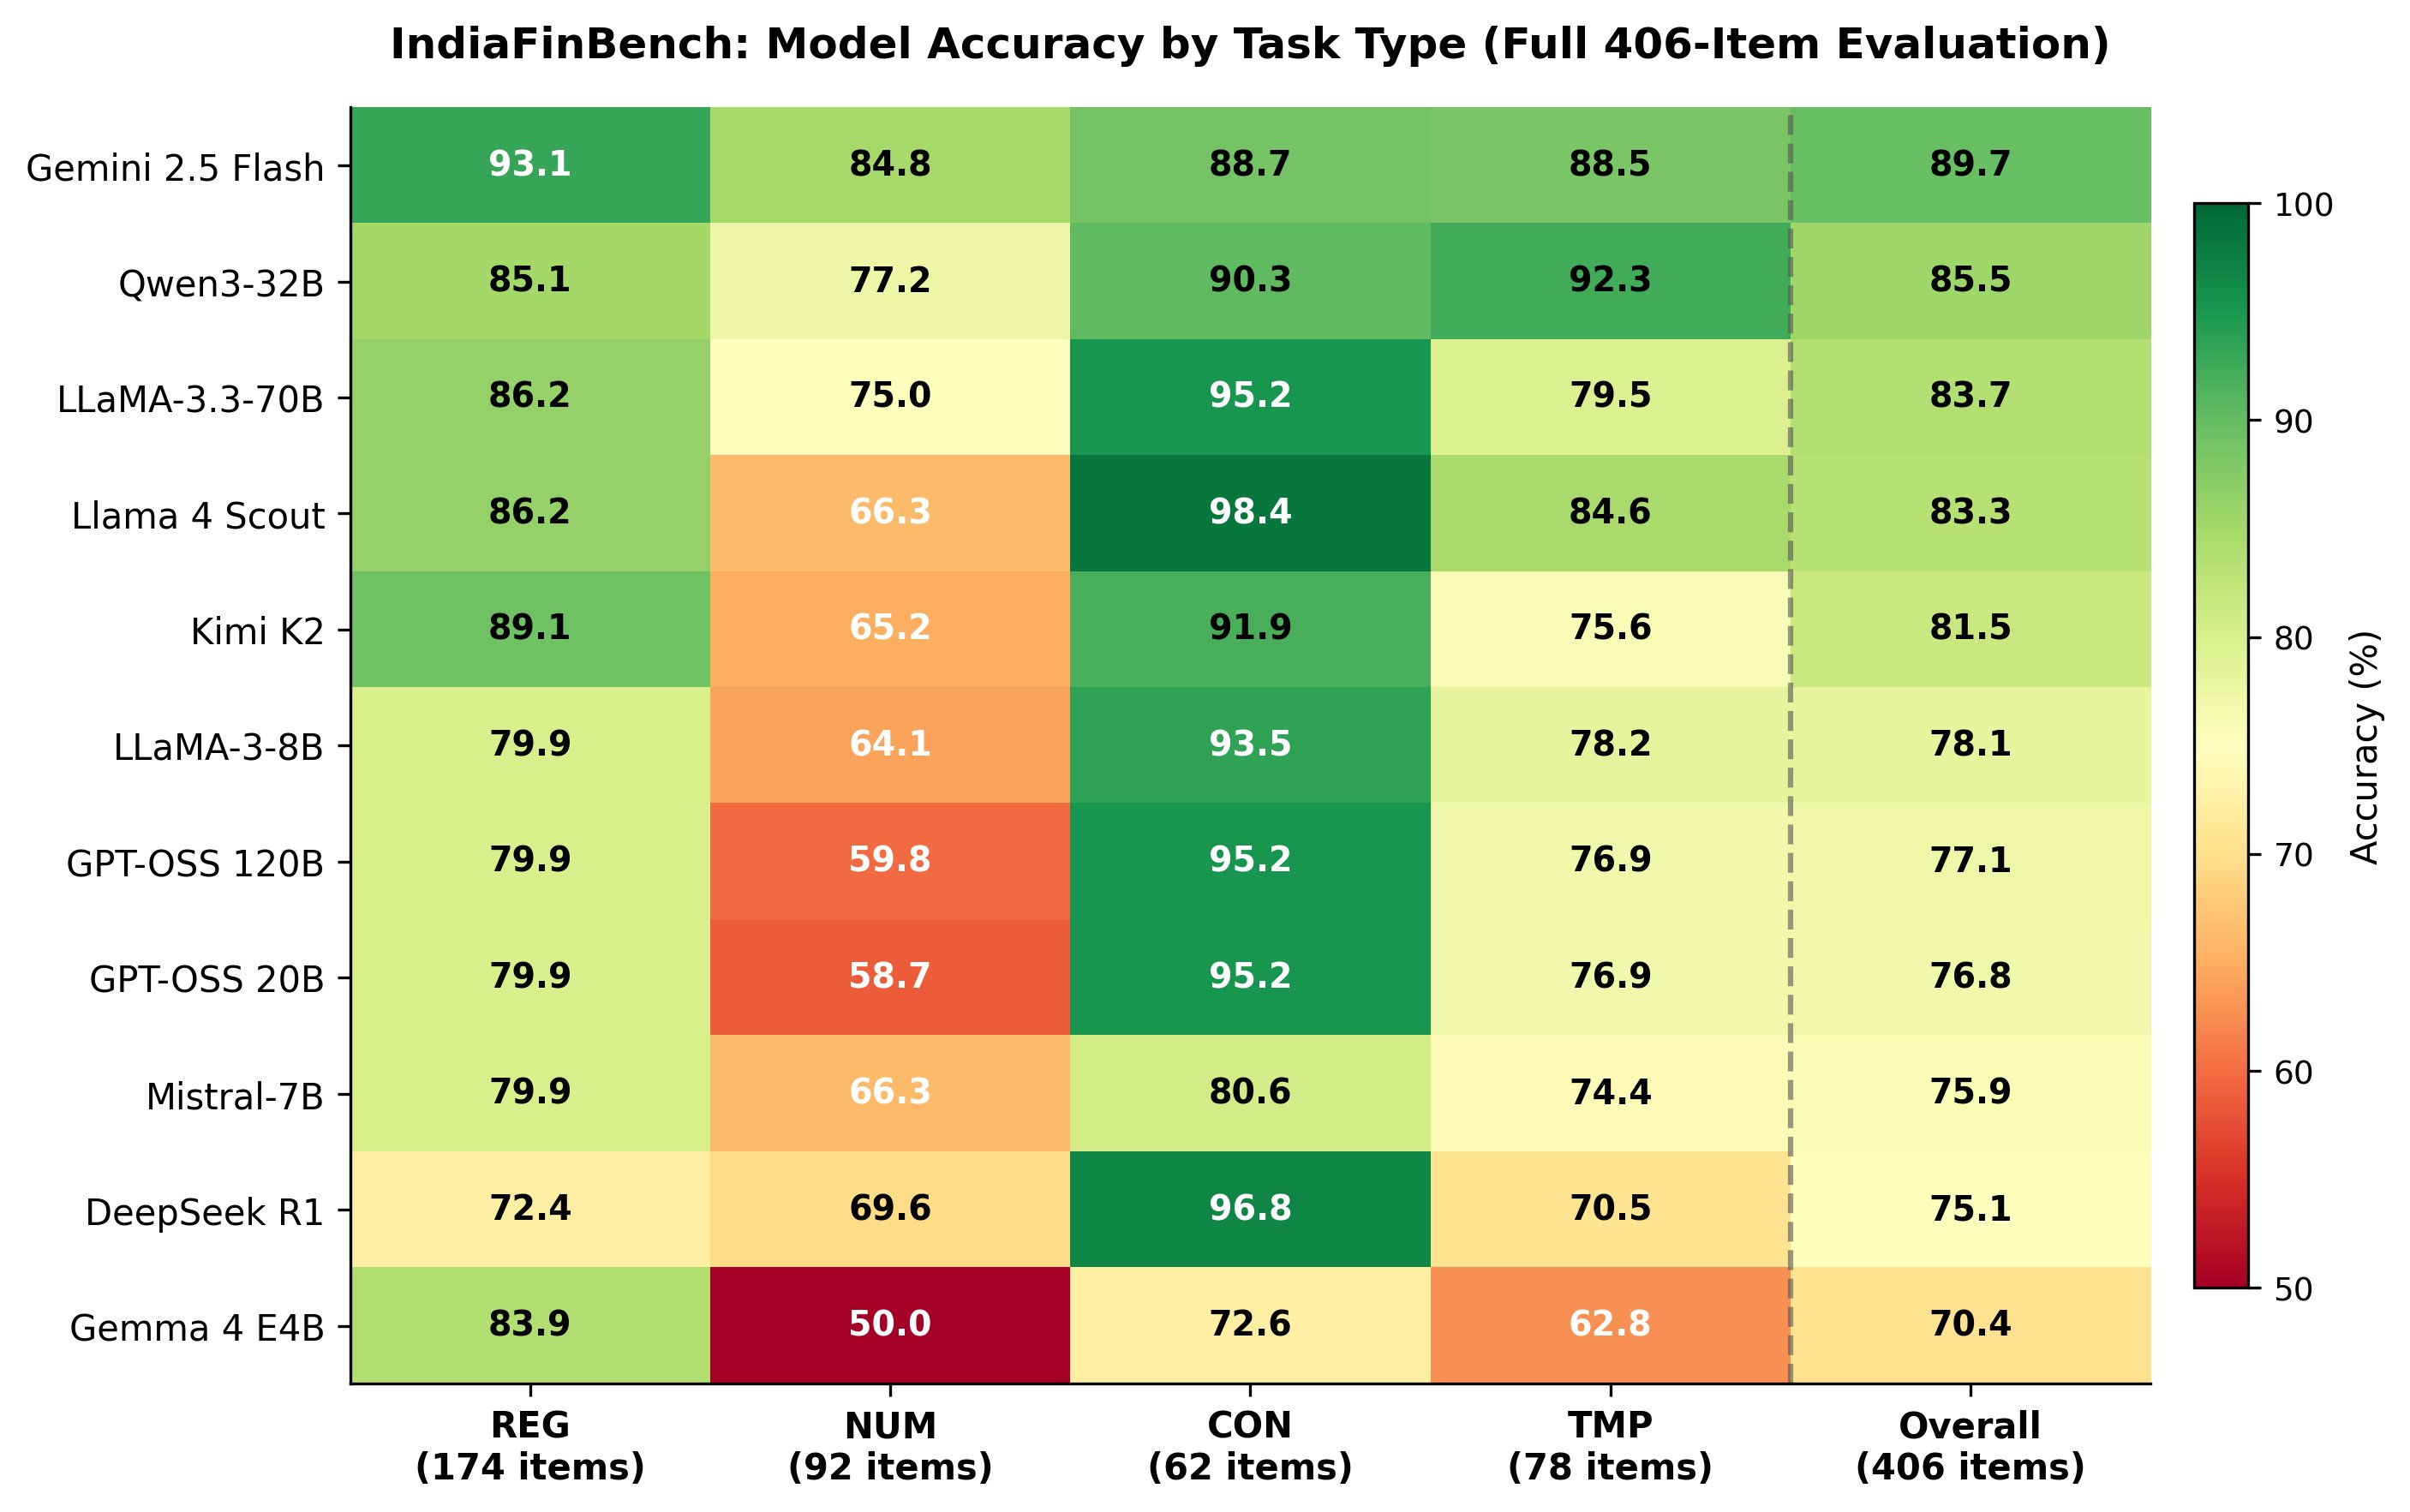
\includegraphics[width=\columnwidth]{figures/fig_heatmap.png}
\caption{Performance heatmap across all twelve models and four task types under strict scoring. Darker cells indicate higher accuracy.}
\label{fig:heatmap}
\end{figure}

\paragraph{Representative failure examples.}

\textbf{Domain Knowledge Failure (Gemma 4 E4B, Regulatory Interpretation).} Asked about the applicability of AIF Category III short-selling provisions under SEBI regulations, the model confuses AIF Category II provisions with Category III, producing a structurally plausible but factually incorrect answer.

\textbf{Numerical Reasoning Failure (GPT-OSS 120B, Numerical Reasoning).} Given an RBI calculation requiring the maximum eligible dividend as a percentage of adjusted PAT, the model correctly identifies the relevant table but applies the wrong conditional threshold, computing the dividend at a higher rate than is warranted by the given capital ratio.

\textbf{Temporal Reasoning Failure (DeepSeek R1 70B, Temporal Reasoning).} Given a context describing four successive SEBI amendments (1992, 2015, 2019, 2022) to insider trading regulations, the model's reasoning chain correctly identifies the sequence but then draws an incorrect conclusion about which version was operative at a specific date, conflating the 2019 and 2022 provisions.

\textbf{Context Grounding Failure (LLaMA-3.3-70B, Contradiction Detection).} Given two RBI passages specifying the same 5\% non-competitive bidding allocation limit in different phrasing (`five per cent' vs.\ `5\%'), the model incorrectly identifies a contradiction based on surface-level differences rather than recognizing semantic equivalence.

\section{Difficulty Breakdown and Task Profiles}
\label{app:difficulty}

Table~\ref{tab:difficulty} reports per-model accuracy by difficulty level; Figure~\ref{fig:difficulty} plots the trajectories, Figure~\ref{fig:radar} shows per-task accuracy profiles, and Figure~\ref{fig:correlation} gives the inter-task correlation structure.

\begin{figure}[t]
\centering
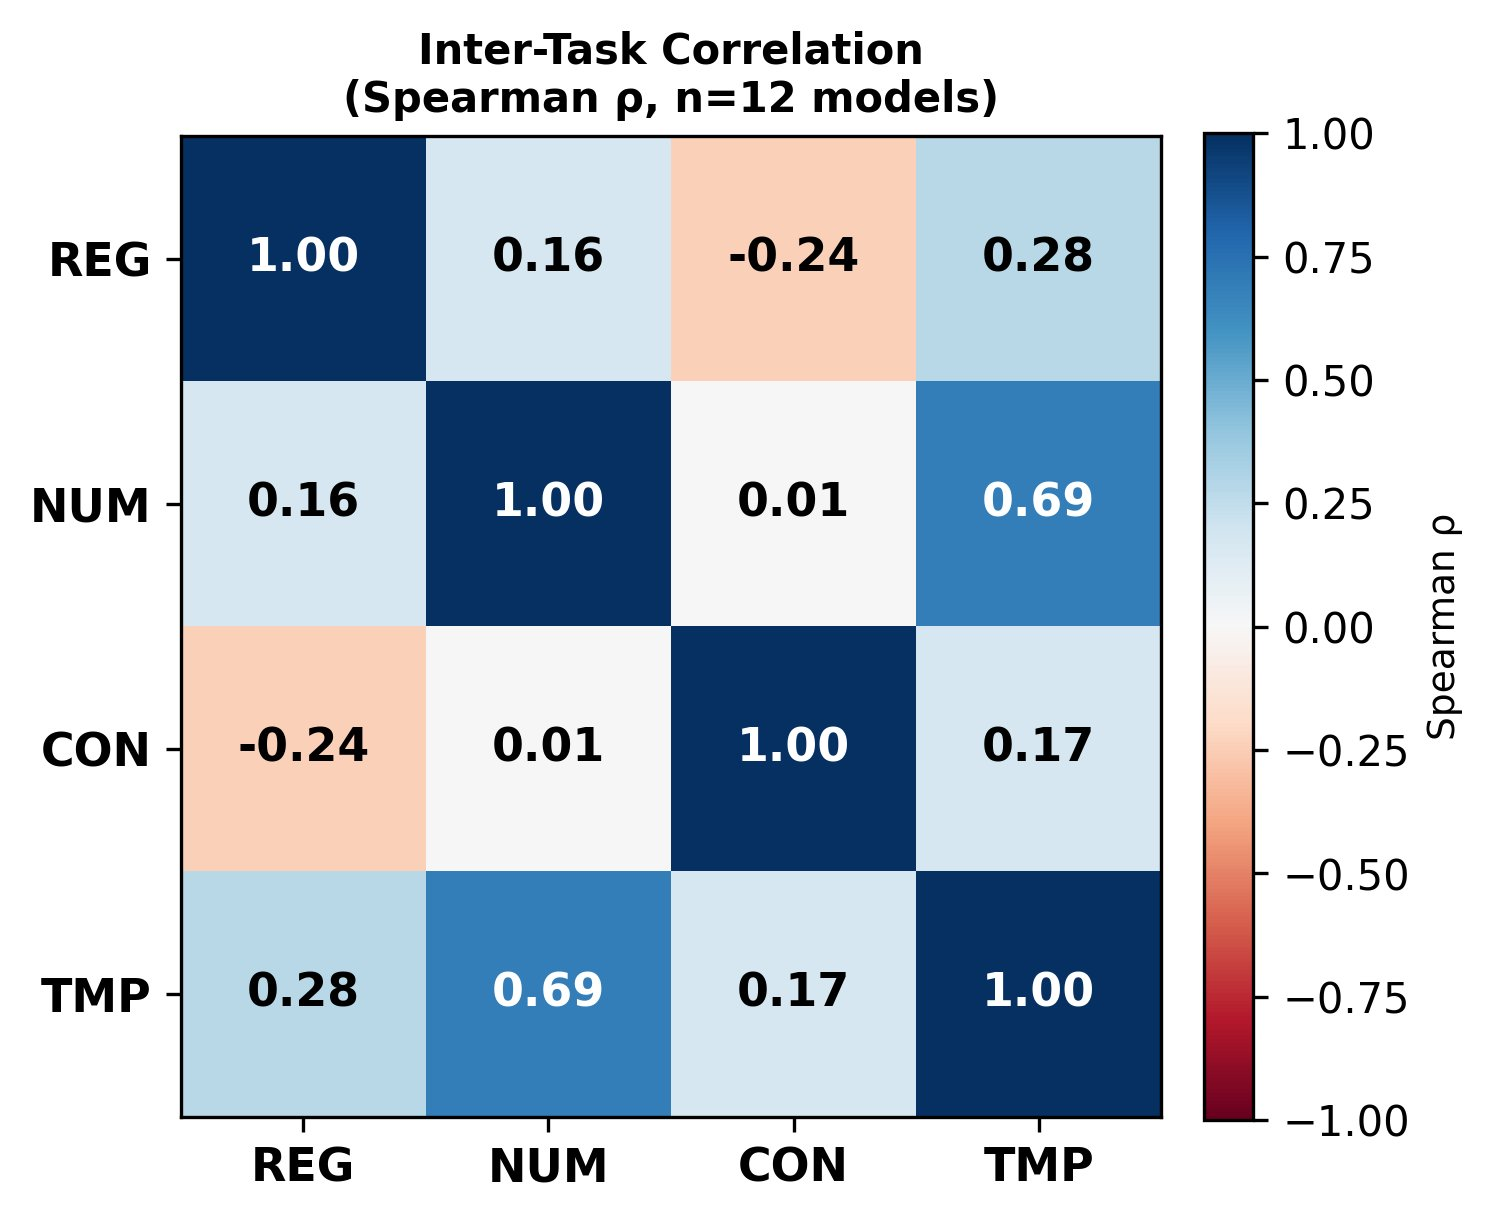
\includegraphics[width=\columnwidth]{figures/fig_correlation.png}
\caption{Inter-task correlation matrix across the four task types. Values indicate Spearman $\rho$ correlation of per-model accuracy vectors across tasks (n=12 models). With n=12, the critical $\rho$ for significance at p$<$0.05 (two-tailed) is approximately 0.58; only the NUM--TMP correlation ($\rho$=0.69) reaches this threshold.}
\label{fig:correlation}
\end{figure}

\begin{table}[t]
\centering\footnotesize
\begin{tabular}{lrrr}
\toprule
\textbf{Model} & \textbf{Easy} & \textbf{Med.} & \textbf{Hard} \\
 & \textit{(n=160)} & \textit{(n=182)} & \textit{(n=64)} \\
\midrule
Gemini 2.5 Flash & 92.5 & 89.0 & 84.4 \\
Qwen3-32B & 81.9 & 87.9 & 87.5 \\
LLaMA-3.3-70B & 79.4 & 85.2 & 90.6 \\
Llama 4 Scout 17B & 82.5 & 81.9 & 89.1 \\
Kimi K2 & 81.9 & 80.8 & 82.8 \\
LLaMA-3-8B & 76.2 & 79.7 & 78.1 \\
GPT-OSS 120B & 79.4 & 76.4 & 73.4 \\
GPT-OSS 20B & 75.0 & 79.7 & 73.4 \\
Gemini 2.5 Pro\textdagger{} & 83.1 & 72.5 & 68.8 \\
Mistral-7B & 74.4 & 76.9 & 76.6 \\
DeepSeek R1 70B & 72.5 & 77.5 & 75.0 \\
Gemma 4 E4B & 82.5 & 64.8 & 56.2 \\
\bottomrule
\end{tabular}
\caption{Accuracy (\%) by difficulty level (full 406-item evaluation, strict pipeline). \textdagger{}Verbose-output scoring artifact; see Appendix~\ref{app:judge}.}
\label{tab:difficulty}
\end{table}

\begin{figure*}[t]
\centering
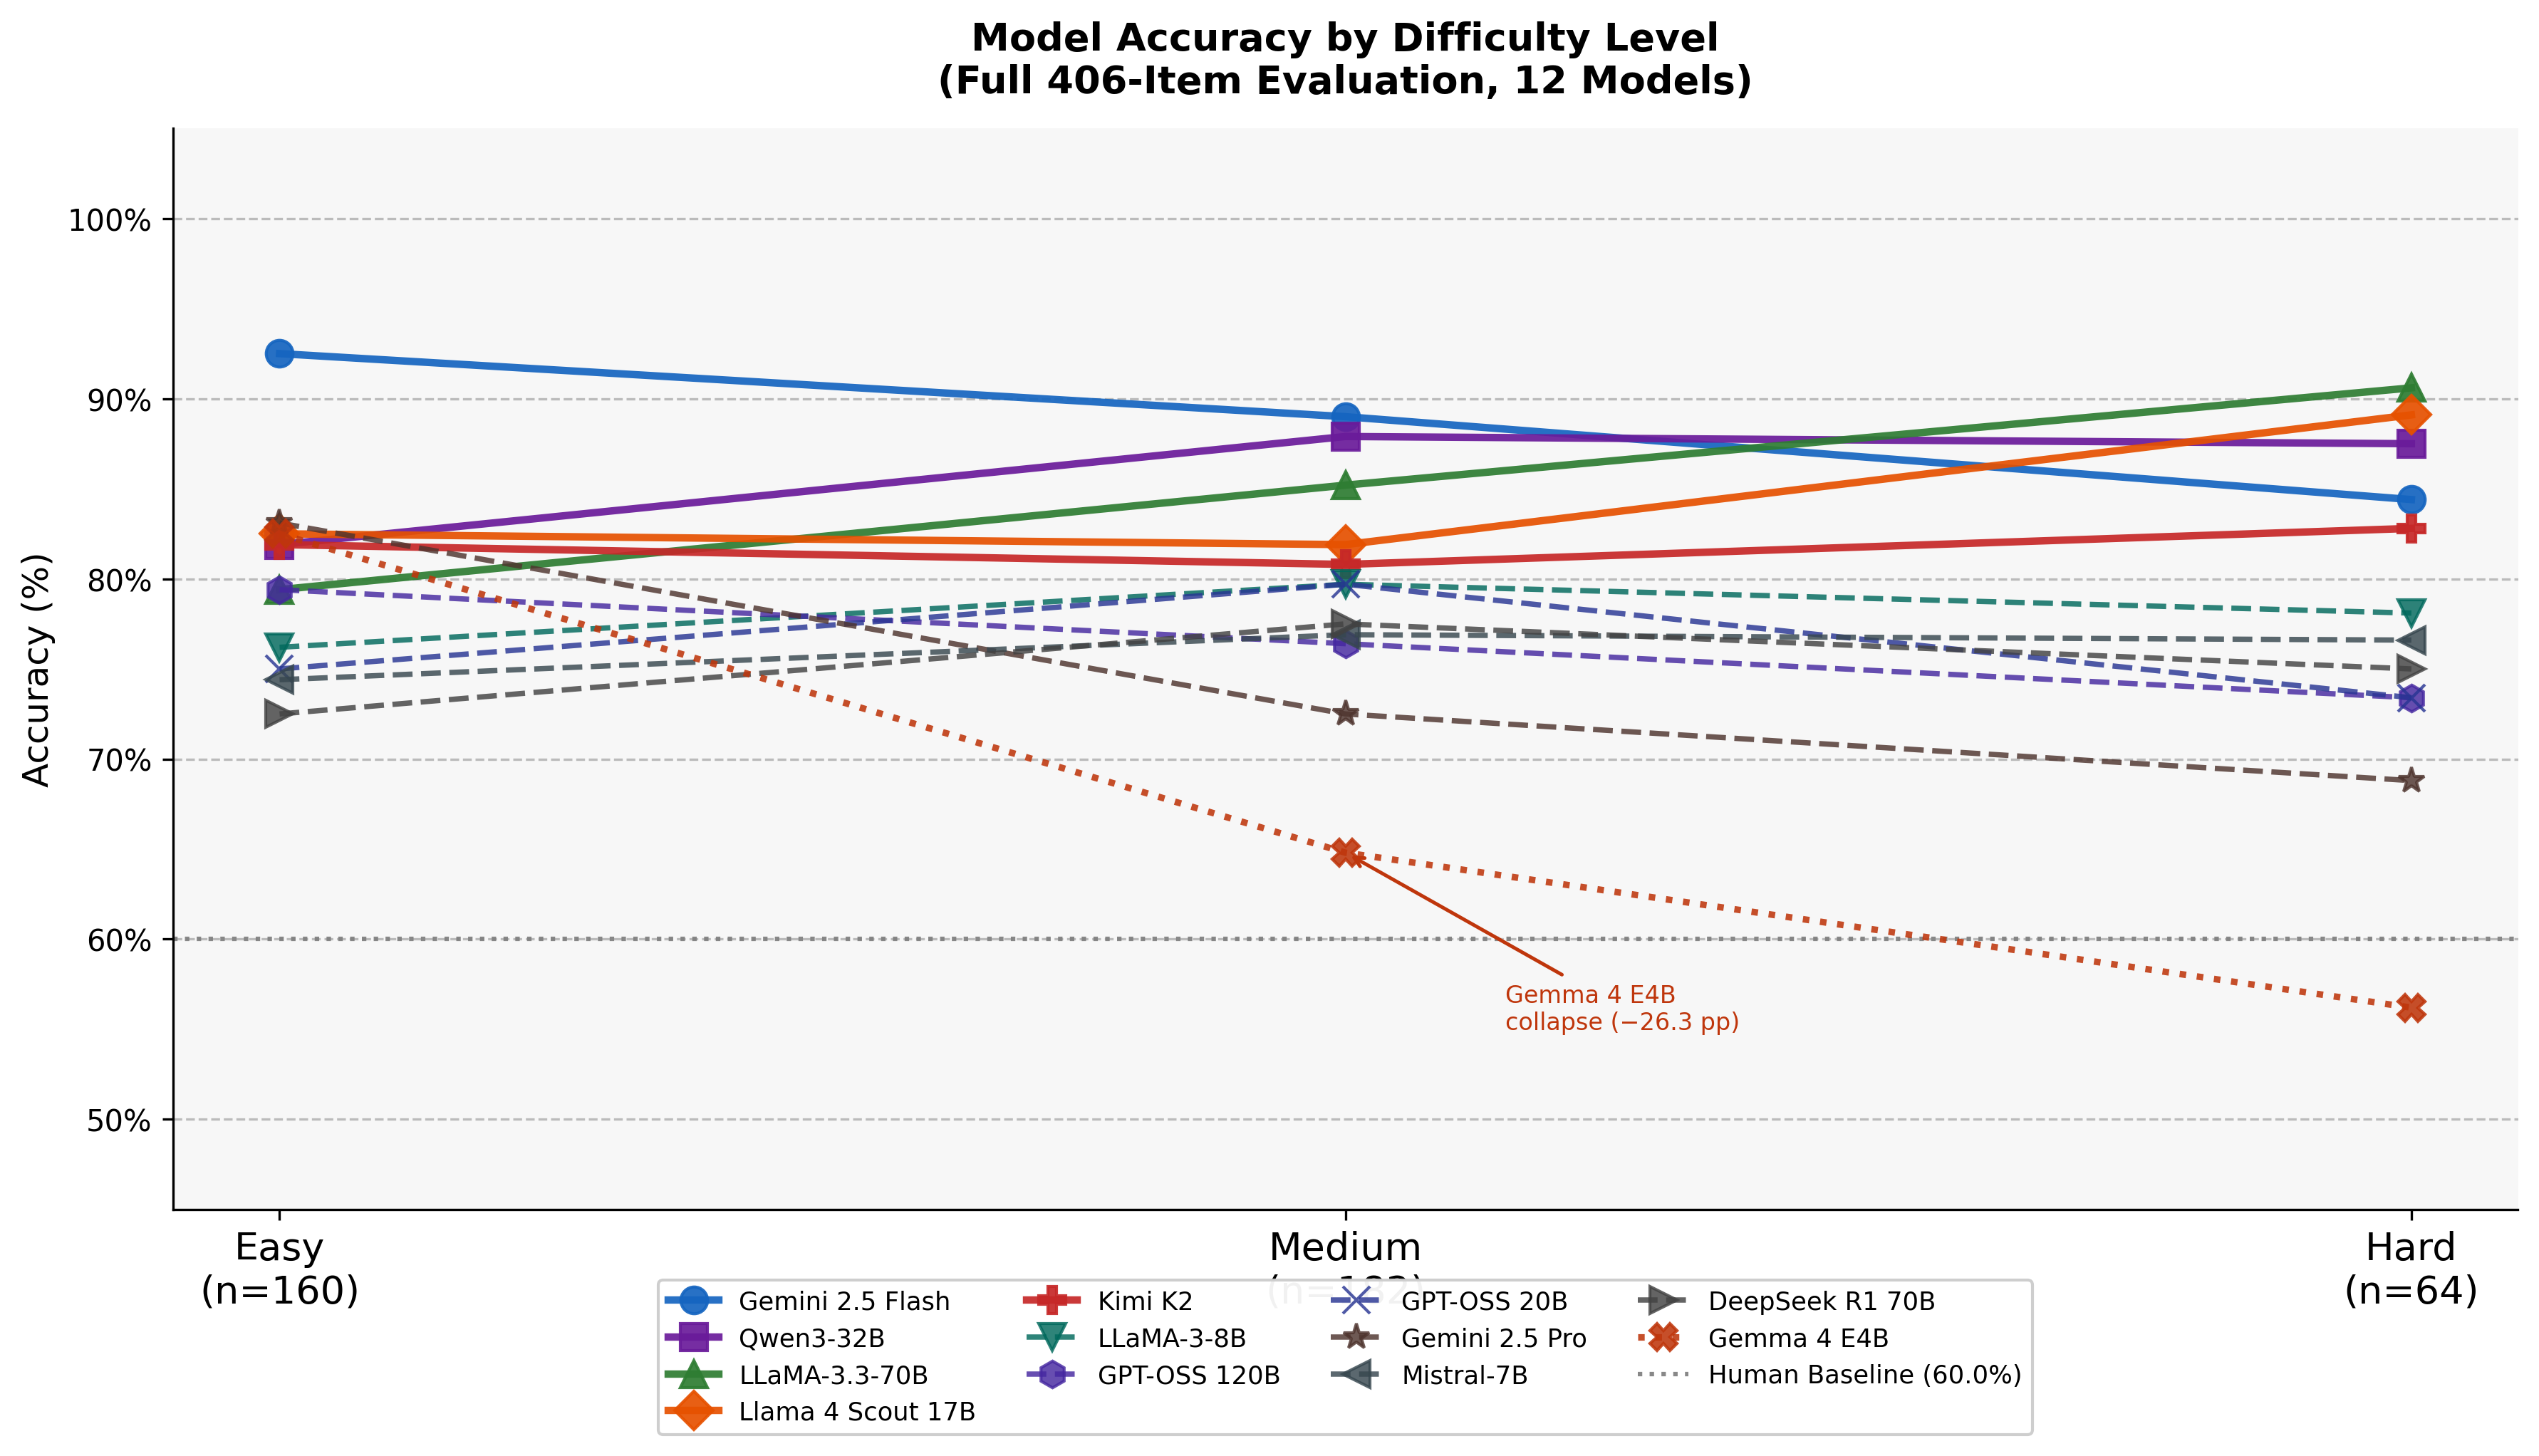
\includegraphics[width=0.75\textwidth]{figures/fig_difficulty.png}
\caption{Per-model accuracy across difficulty levels (Easy / Medium / Hard). Lines connect the three difficulty conditions for each model.}
\label{fig:difficulty}
\end{figure*}

\begin{figure}[t]
\centering
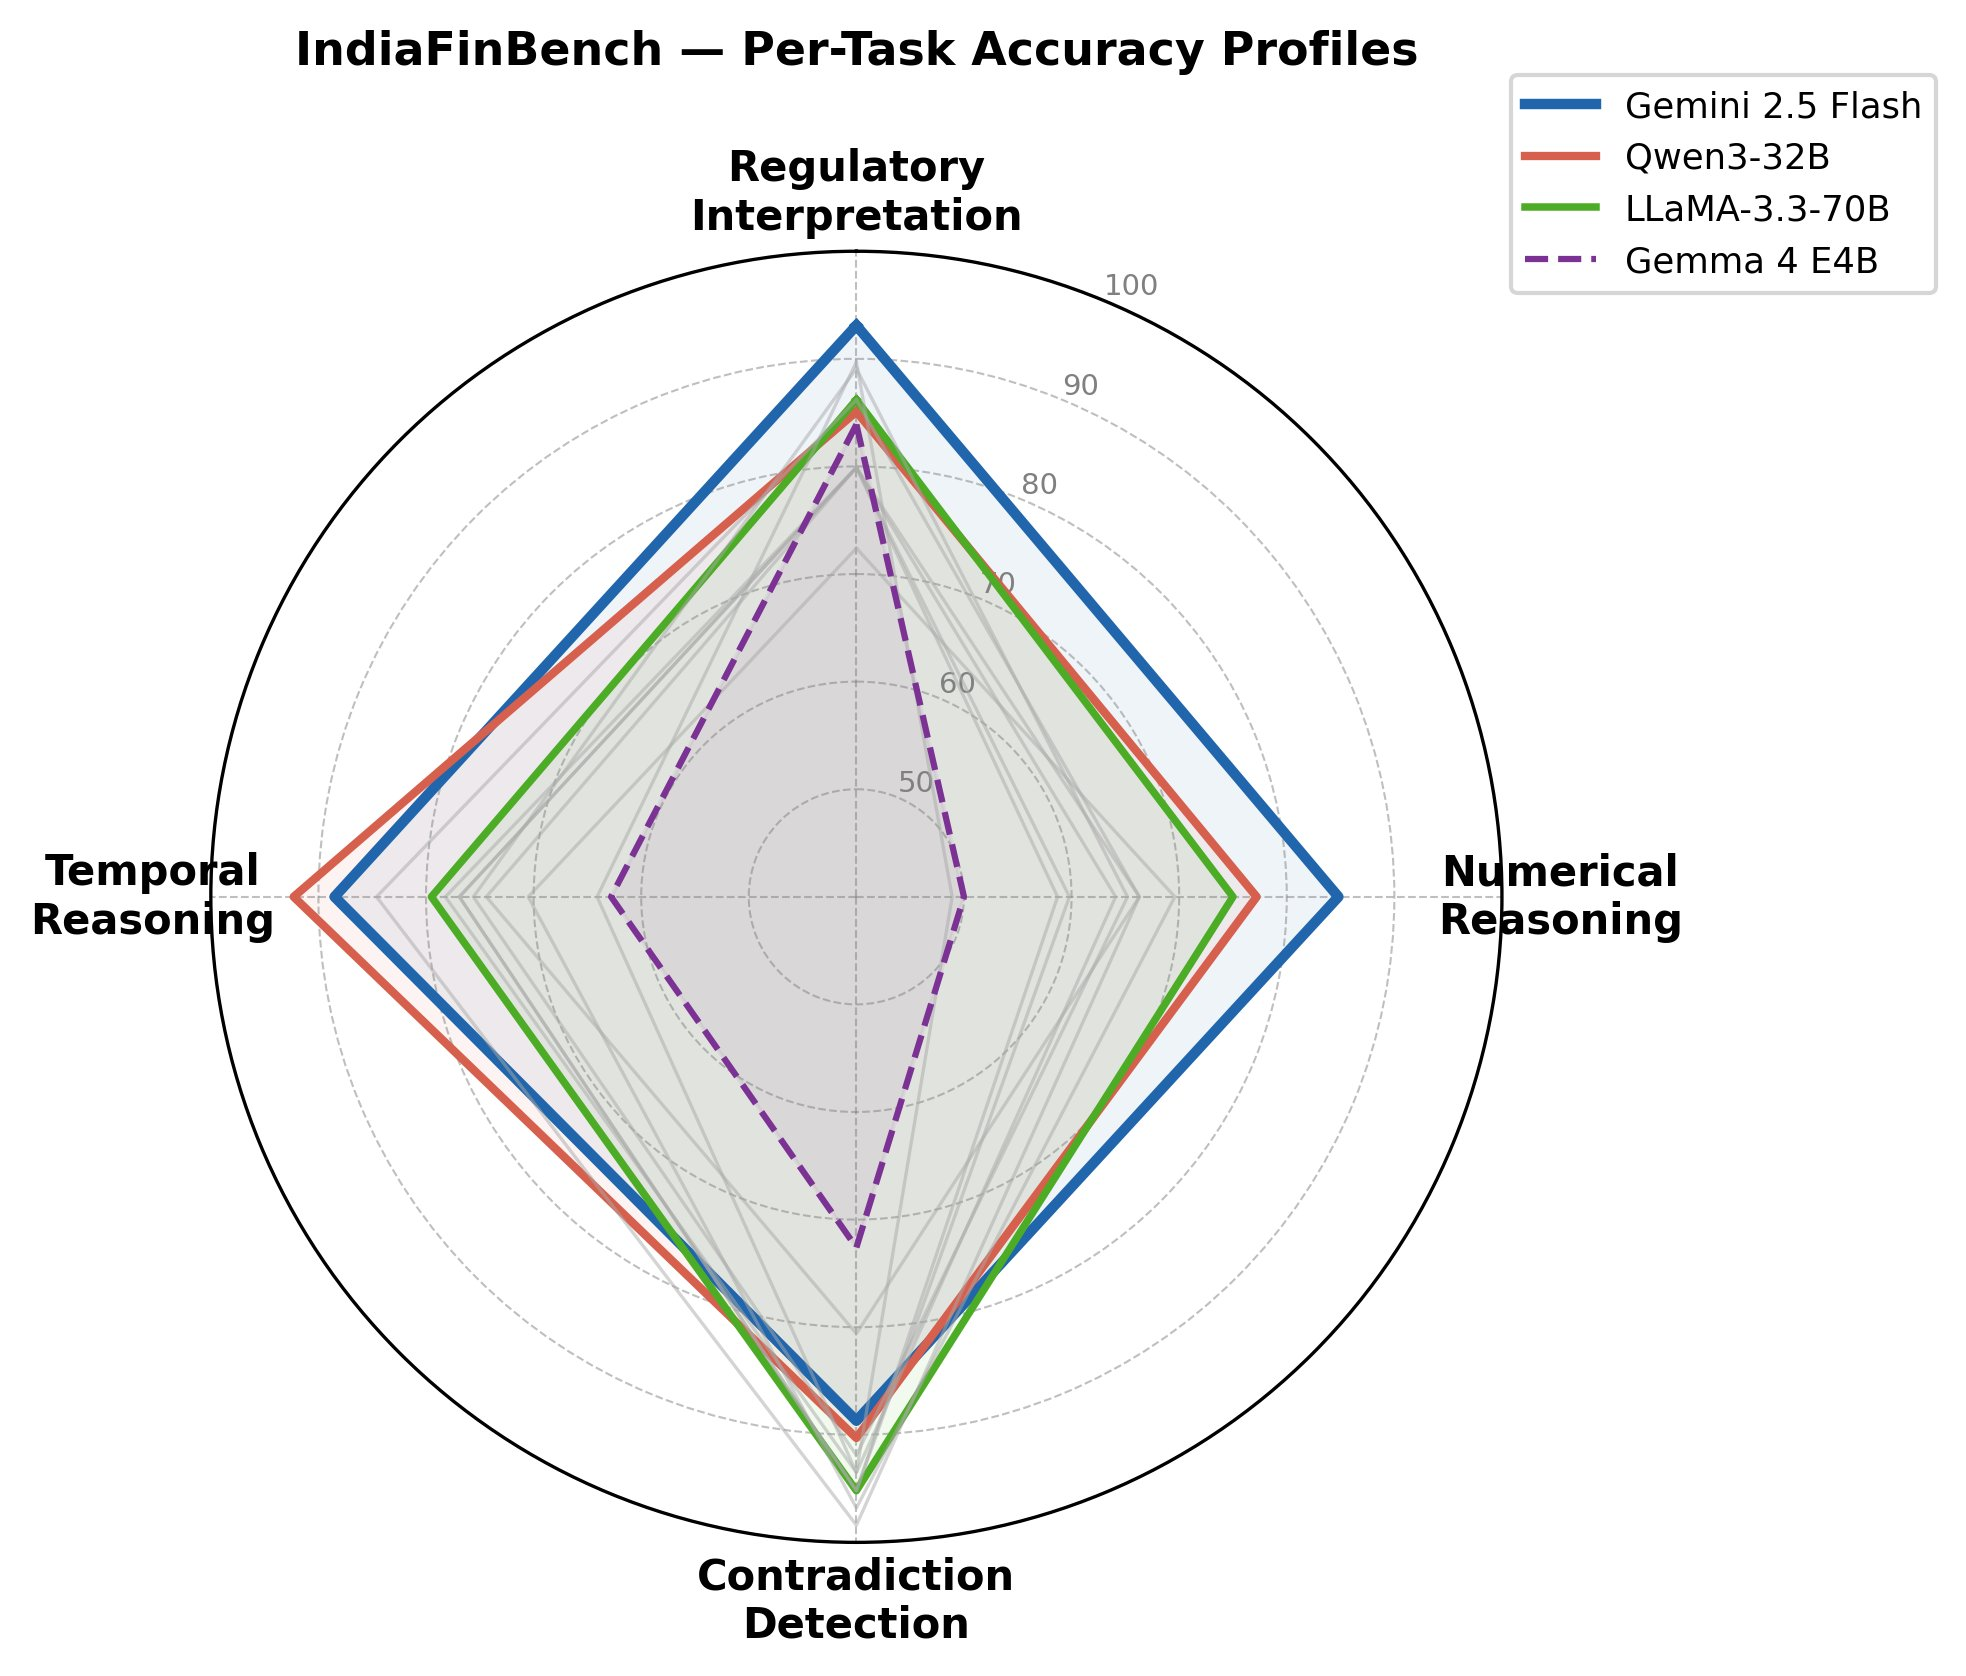
\includegraphics[width=\columnwidth]{figures/fig_radar.png}
\caption{Radar chart comparing per-task accuracy profiles across models. Each axis represents a task type.}
\label{fig:radar}
\end{figure}

\section{Few-Shot Evaluation}
\label{app:fewshot}

To assess whether zero-shot evaluation represents a conservative lower bound on model capability, we evaluated four top-performing models---Gemini 2.5 Flash, LLaMA-3.3-70B, Llama 4 Scout 17B, and Qwen3-32B---under 3-shot prompting. For each task type, three fixed in-context examples were prepended to the prompt, drawn from the same distribution as the benchmark items and held constant across all models. All other evaluation conditions (system prompt, scoring pipeline, dataset) were identical to the zero-shot setup.

\begin{table*}[t]
\centering\small
\begin{tabular}{llrrrrr}
\toprule
\textbf{Model} & \textbf{Cond.} & \textbf{REG} & \textbf{NUM} & \textbf{CON} & \textbf{TMP} & \textbf{Overall} \\
\midrule
\multirow{3}{*}{Gemini 2.5 Flash} & 0-shot & 93.1\% & 84.8\% & 88.7\% & 88.5\% & 89.7\% \\
 & 3-shot & 92.0\% & 87.0\% & 91.9\% & 88.5\% & 90.1\% \\
 & $\Delta$ & $-$1.1 & +2.2 & +3.2 & +0.0 & +0.4 \\
\midrule
\multirow{3}{*}{Qwen3-32B} & 0-shot & 85.1\% & 77.2\% & 90.3\% & 92.3\% & 85.5\% \\
 & 3-shot & 86.8\% & 79.3\% & 90.3\% & 92.3\% & 86.7\% \\
 & $\Delta$ & +1.7 & +2.1 & +0.0 & +0.0 & +1.2 \\
\midrule
\multirow{3}{*}{LLaMA-3.3-70B} & 0-shot & 86.2\% & 75.0\% & 95.2\% & 79.5\% & 83.7\% \\
 & 3-shot & 87.4\% & 77.2\% & 98.4\% & 87.2\% & 86.7\% \\
 & $\Delta$ & +1.2 & +2.2 & +3.2 & +7.7 & +3.0 \\
\midrule
\multirow{3}{*}{Llama 4 Scout 17B} & 0-shot & 86.2\% & 66.3\% & 98.4\% & 84.6\% & 83.3\% \\
 & 3-shot & 90.2\% & 82.6\% & 85.5\% & 76.9\% & 85.2\% \\
 & $\Delta$ & +4.0 & +16.3 & $-$12.9 & $-$7.7 & +1.9 \\
\bottomrule
\end{tabular}
\caption{Zero-shot vs. 3-shot accuracy by task type.}
\label{tab:e1}
\end{table*}

3-shot prompting improves numerical reasoning by 2.1--16.3 percentage points across all four models, with Llama 4 Scout 17B showing the largest NUM gain (+16.3 pp, from 66.3\% to 82.6\%). LLaMA-3.3-70B gains +7.7 pp on temporal reasoning under 3-shot. These improvements confirm the direction of the zero-shot conservatism claimed in Section~\ref{sec:main-results-text} without altering comparative structure.

CON performance is mixed: Llama 4 Scout 17B declines 12.9 pp (from near-ceiling 98.4\% to 85.5\%), while Gemini 2.5 Flash improves +3.2 pp. Performance degradation under 3-shot on tasks with near-ceiling zero-shot accuracy is consistent with in-context example interference, where the few-shot prefix biases the model away from clear Yes/No responses on straightforward contradiction items. Qwen3-32B is unaffected on CON and TMP (0.0 pp), suggesting its zero-shot behavior is already well-calibrated for these task types.

Overall, the performance tier ordering is preserved under 3-shot prompting (Gemini 2.5 Flash $\geq$ Qwen3-32B $\geq$ LLaMA-3.3-70B $\approx$ Llama 4 Scout 17B), confirming that the tier structure observed in zero-shot evaluation reflects genuine model capability differences rather than prompting strategy sensitivity.

\end{document}
